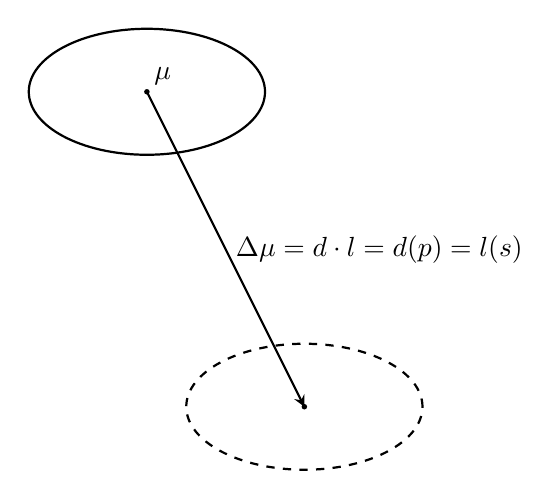
\begin{tikzpicture}
    \def\x{0}
    \def\y{2}
    \def\xf{2}
    \def\yf{-2}
    % Draw the larger ellipse labeled X_μ
    \draw[thick] (\x, \y) ellipse (1.5 and 0.8);
    \node at (\x + 0.2, \y + 0.2) {\textbf{$\mu$}};
    
    % Draw the smaller dashed ellipse labeled "interior"
    \draw[thick, dashed] (\xf, \yf) ellipse (1.5 and 0.8);
    % \node[below] at (0, -2.5) {\textit{interior}};
    
    % Draw points and arrow
    \fill (\x, \y) circle (1pt); % Point at the center of X_μ
    \fill (\xf, \yf) circle (1pt); % Point at the center of interior
    \draw[thick, ->, >=stealth] (\x, \y) -- (\xf, \yf) node[midway, right] {$\Delta \mu = d \cdot l = d (p) = l(s)$};
    
    % Annotate components of the formula
    % \node[right] at (\xf, \yf + 1) {$d$ (growth direction probabilities)};
    % \node[right] at (\xf, \yf + 0.5) {$l(s)$};
\end{tikzpicture}